\documentclass[11pt,a4paper]{ctexart}

\usepackage[margin=2.4cm]{geometry}
\usepackage{amsmath,amssymb}
\usepackage{graphicx}
\usepackage{booktabs}
\usepackage{float}
\usepackage{xcolor}
\usepackage{caption}
\usepackage{tikz}
\usetikzlibrary{arrows.meta}
\usepackage{listings}
\usepackage[hidelinks]{hyperref}

\setCJKmainfont{Noto Serif CJK SC}
\setCJKsansfont{Noto Sans CJK SC}
\setCJKmonofont{Noto Sans Mono CJK SC}

\captionsetup{font=small,labelfont=bf}
\lstset{basicstyle=\ttfamily\small,frame=single,breaklines=true,
        columns=fullflexible,keepspaces=true,showstringspaces=false}

\title{\textbf{Computer Vision (2026 Fall) --- Homework 1}}
\author{姓名：石禾言 \qquad 学号：2500013221}
\date{2026 年 9 月}

\begin{document}
\maketitle

\section{简答题}

\subsection{齐次坐标}

\paragraph{1) 表示同一个笛卡尔点的充要条件与笛卡尔坐标}

设 $\mathbf p=(p_1,\dots,p_N,s)$，$\mathbf q=(q_1,\dots,q_N,t)$，其中 $s,t\neq 0$。
对 $\mathbf p$ 作归一化，得 $\bar{\mathbf p}=(p_1/s,\dots,p_N/s,1)$；
对 $\mathbf q$ 同理得 $\bar{\mathbf q}=(q_1/t,\dots,q_N/t,1)$。

$\mathbf p$ 与 $\mathbf q$ 表示同一个笛卡尔点，当且仅当它们的归一化表示完全相同，即
\begin{equation}
\bar{\mathbf p}=\bar{\mathbf q}
\iff \frac{p_i}{s}=\frac{q_i}{t}\ \ (i=1,\dots,N)
\iff t\,p_i=s\,q_i\ \ (i=1,\dots,N)
\iff \exists\,\lambda\neq 0:\ \mathbf p=\lambda\,\mathbf q,
\end{equation}
其中 $\lambda=s/t$。也就是说，\textbf{充要条件是两个齐次坐标向量成比例}（$s,t\neq 0$）。
该点对应的笛卡尔坐标为 $\bigl(p_1/s,\ p_2/s,\ \dots,\ p_N/s\bigr)$。

这说明齐次坐标表示\textbf{不唯一}：同一个点对应同一条过原点直线上的无穷多个非零向量，相差一个非零比例因子。

\paragraph{2) 齐次坐标的两个优点}

\textbf{优点一：把平移与线性变换统一成同一个矩阵乘法。}
在笛卡尔坐标下，仿射变换必须写成 $N$ 维空间中的“线性变换 $+$ 平移”
$\mathbf x\mapsto A\mathbf x+\mathbf b$，它不是 $\mathbb R^N$ 上的线性映射，无法用一个 $N\times N$ 矩阵表示，
复合、求逆都要单独处理平移分量。改用齐次坐标后，同一个变换写成
\begin{equation}
\begin{bmatrix}\mathbf x'\\ 1\end{bmatrix}
=\begin{bmatrix}A&\mathbf b\\ \mathbf 0^\top &1\end{bmatrix}
\begin{bmatrix}\mathbf x\\ 1\end{bmatrix},
\end{equation}
即一个 $(N{+}1)\times(N{+}1)$ 矩阵的乘法。于是所有仿射变换（含平移、旋转、缩放、错切）都成为同一个线性空间上的线性算子，
变换的复合就是矩阵相乘；当变换可逆时，求逆就是矩阵求逆。

\textbf{优点二：可以统一表示无穷远点（方向）。}
当 $s=0$ 且 $(p_1,\dots,p_N)\neq\mathbf 0$ 时，齐次向量 $(p_1,\dots,p_N,0)$ 不对应任何有限笛卡尔点，它表示该方向上的\textbf{无穷远点}。
在齐次坐标框架下：
(i) 平行直线也有交点——它们交于无穷远点，因此“射影平面内任意两条不同直线必相交”无需对平行情形作例外讨论；
(ii) 相机的投影可以写成齐次线性映射，图像的\textbf{消失点/消失线}可以自然表示出来；
(iii) 投影变换可以把无穷远线映射为一条有限直线，实现自由转换。

\subsection{卷帘快门}

设行曝光时间为 $\Delta t_{\text{row}}=T/H$，第 $y$ 行的曝光时刻为 $t(y)=y\,\Delta t_{\text{row}}$（$y$ 自上而下增大），
因此\textbf{图像下方的行曝光更晚}。

\paragraph{1) 列车运动方向的判断}

在卷帘快门图像（图 1 下）中，车门竖直边的下端比上端向\textbf{左}偏移了 $X=200$ 像素。
下端所在的行曝光得更晚，即在下端被曝光的时刻，列车（以及车门边）已经相对上端被曝光的时刻向图像左侧移动了 $200$ 像素。
因此\textbf{列车向左运动}。

\begin{figure}[H]
\centering
\begin{tikzpicture}[x=1.15cm,y=1.15cm,>=Stealth]
  % sheared door edge
  \draw[very thick,orange] (2.4,0) -- (0,-2.0);
  \draw[very thick,orange] (0,0) -- (2.4,0);      % X leg
  \draw[very thick,orange] (0,0) -- (0,-2.0);     % Y leg
  \draw[dashed,gray] (2.4,0) -- (2.4,-2.0);
  \draw[dashed,gray] (0,-2.0) -- (2.4,-2.0);
  % scan direction
  \draw[->,thick,blue] (-1.1,0.25) -- (-1.1,-2.25);
  \node[blue,rotate=90,font=\small] at (-1.55,-1.0) {行曝光方向};
  \foreach \y in {0,-0.4,...,-2.0} \draw[blue] (-1.25,\y) -- (-0.95,\y);
  % labels
  \node[above,font=\small] at (1.2,0.05) {$X=200$ px};
  \node[font=\small,anchor=west,fill=white,inner sep=1.5pt] at (0.12,-1.0) {$Y=300$ px};
  \node[font=\small,align=left,anchor=west] at (2.6,-1.0)
      {卷帘快门下的\\车门竖直边\\(上端靠右、下端靠左)};
\end{tikzpicture}
\caption{卷帘快门造成的竖直边倾斜（对应题目图 1 下半幅）。竖直边的上端曝光更早、下端更晚，
两者水平相差 $X=200$ px、竖直相差 $Y=300$ px；由图中的倾斜方向（上右下左）可知列车向左运动。}
\end{figure}

\paragraph{2) 列车速度的计算}

行曝光时间
\begin{equation}
\Delta t_{\text{row}}=\frac{T}{H}=\frac{30\ \text{ms}}{1000}=0.03\ \text{ms/row}.
\end{equation}
车门边两端所对应的曝光时间差（即曝光完这 $Y=300$ 行所需的时间）
\begin{equation}
\Delta t=Y\cdot\Delta t_{\text{row}}=300\times 0.03\ \text{ms}=9\ \text{ms}=9\times10^{-3}\ \text{s}.
\end{equation}
在这段时间里，车门边在像面上水平移动了 $X$ 像素。由针孔模型，像面上 $x$ 方向的位移 $\Delta x'$ 与深度 $Z$ 处的真实位移 $\Delta X_{\text{real}}$ 满足
$\Delta X_{\text{real}}=\Delta x'\cdot Z/f$，于是
\begin{equation}
\Delta X_{\text{real}}=X\cdot\frac{Z}{f_x}=200\times\frac{15\ \text{m}}{6000}=0.5\ \text{m}.
\end{equation}
列车速度
\begin{equation}
v=\frac{\Delta X_{\text{real}}}{\Delta t}=\frac{0.5\ \text{m}}{9\times10^{-3}\ \text{s}}
=55.6\ \text{m/s}\approx 2.0\times10^{2}\ \text{km/h},
\end{equation}
方向为\textbf{水平向左}（与第 1) 问一致）。合并起来即
\begin{equation}
v=\frac{X\,Z}{f_x\,Y\,\Delta t_{\text{row}}}=\frac{X\,Z\,H}{f_x\,Y\,T}
=\frac{200\times15\times1000}{6000\times300\times30\times10^{-3}}=55.6\ \text{m/s}.
\end{equation}

\clearpage
\section{相机高度}

\subsection{求消失线}

\textbf{测量依据。} 在原始 \texttt{campus.png}（$4096\times3072$）上选择地面铺装的两个方向。
坐标原点为图像左上角，$x$ 向右、$y$ 向下，以下坐标均为原图像素坐标。
纵深组 $D_1,D_2$ 是广场铺装中两条相隔较远、沿街道纵深排列的接缝；
横向组 $T_1,T_2$ 分别为铺装与道路之间的直线边界及其后方的一条横向铺装接缝。
同组线在地面上近似平行，两个方向不同。避开黄色坐标轴、人物和花坛遮挡处，
沿可见接缝的暗色像素搜索直线位置；断续接缝按同一直线拟合。
表 \ref{tab:q2lines} 的两端点表示拟合后的线段，保留小数仅为方便复算，不表示亚像素测量精度。
图 \ref{fig:q2measure} 展示所选线段。

\begin{table}[H]
\centering
\caption{原图上两组平行线的拟合线段端点（单位：像素）。}
\label{tab:q2lines}
\begin{tabular}{clll}
\toprule
方向 & 线段 & 端点 $P$ & 端点 $Q$\\
\midrule
纵深 & $D_1$ & $(2167.02,\ 2170)$ & $(2113.00,\ 2355)$\\
纵深 & $D_2$ & $(2836.99,\ 2170)$ & $(3086.00,\ 2355)$\\
横向 & $T_1$ & $(1900,\ 2374.750)$ & $(4000,\ 2350.600)$\\
横向 & $T_2$ & $(1900,\ 2272.875)$ & $(4000,\ 2246.100)$\\
\bottomrule
\end{tabular}
\end{table}

\textbf{消失点计算。} 将端点写成齐次坐标 $\tilde P=(x_P,y_P,1)^\top$，
直线为 $\ell=\tilde P\times\tilde Q$。由表中端点得到
\begin{equation}
\begin{aligned}
D_1 &: x+0.292y-2800.66=0, & D_2 &: x-1.346y+83.83=0,\\
T_1 &: 0.0115x+y-2396.60=0, & T_2 &: 0.01275x+y-2297.10=0.
\end{aligned}
\end{equation}
同组直线的交点 $V_D=\ell_{D_1}\times\ell_{D_2}$、$V_T=\ell_{T_1}\times\ell_{T_2}$
归一化后为
\begin{equation}
V_D\approx(2286.45,\ 1760.98,\ 1)^\top,\qquad
V_T\approx(-79600,\ 3312,\ 1)^\top.
\end{equation}

\textbf{消失线。} 两个方向都属于地面平面，故 $\ell_h=V_D\times V_T$。
归一化令 $y$ 的系数为 $1$，得到
\begin{equation}
\boxed{\ \ell_h:\ 0.0189411x+y-1804.2908=0,
\quad\text{即 }y=-0.0189411x+1804.2908.\ }
\end{equation}
将两个消失点代回此式，均满足直线方程。消失线轻微倾斜，约 $1.09^\circ$，
因此使用花坛所在位置的消失线纵坐标。

\begin{figure}[H]
\centering
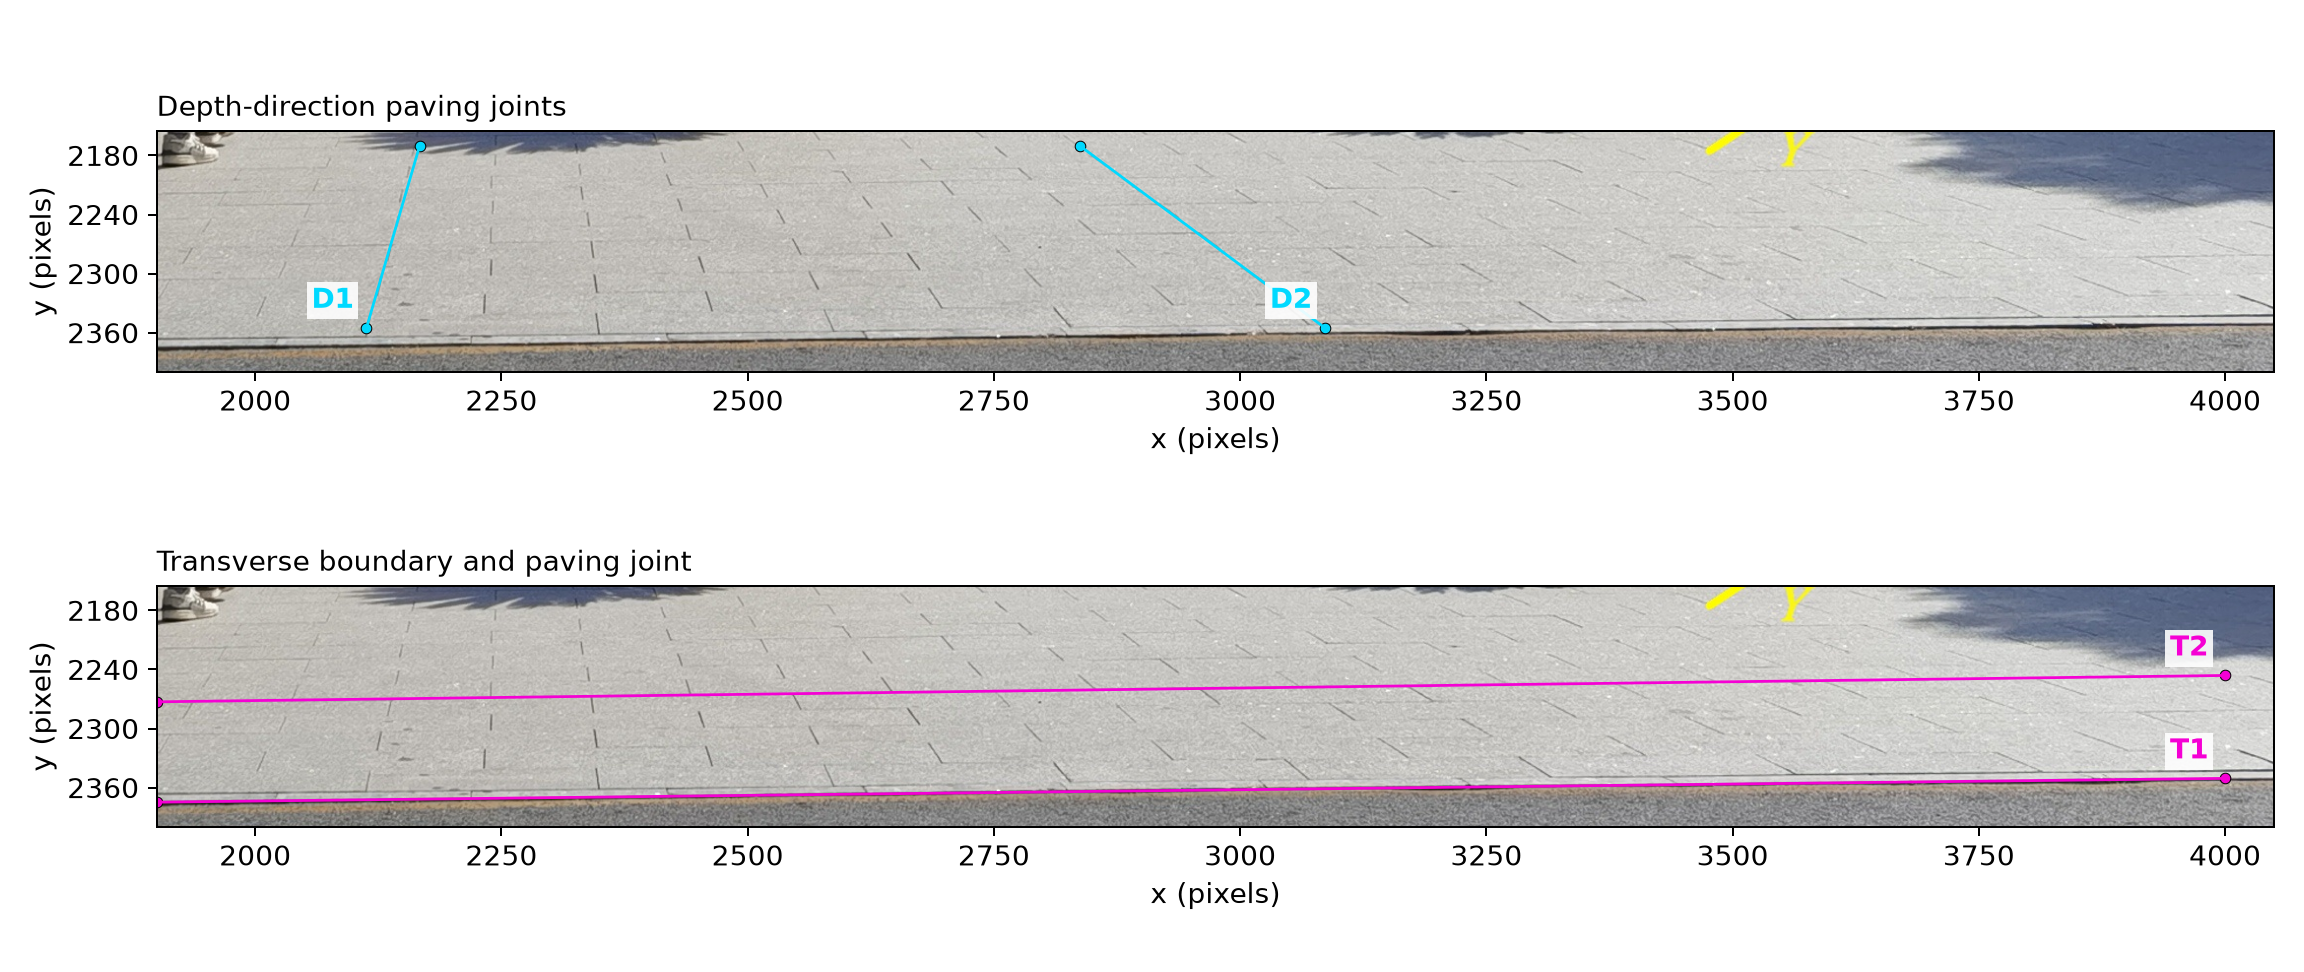
\includegraphics[width=\textwidth]{figs/q2_line_measurements.png}
\caption{原图地面区域的测量细节。上图青色为纵深方向的 $D_1,D_2$；下图品红色为横向的 $T_1,T_2$。
彩色端点对应表 \ref{tab:q2lines}。原图中的黄色线是题目已有的坐标示意，不参与测量。}
\label{fig:q2measure}
\end{figure}

\begin{figure}[H]
\centering
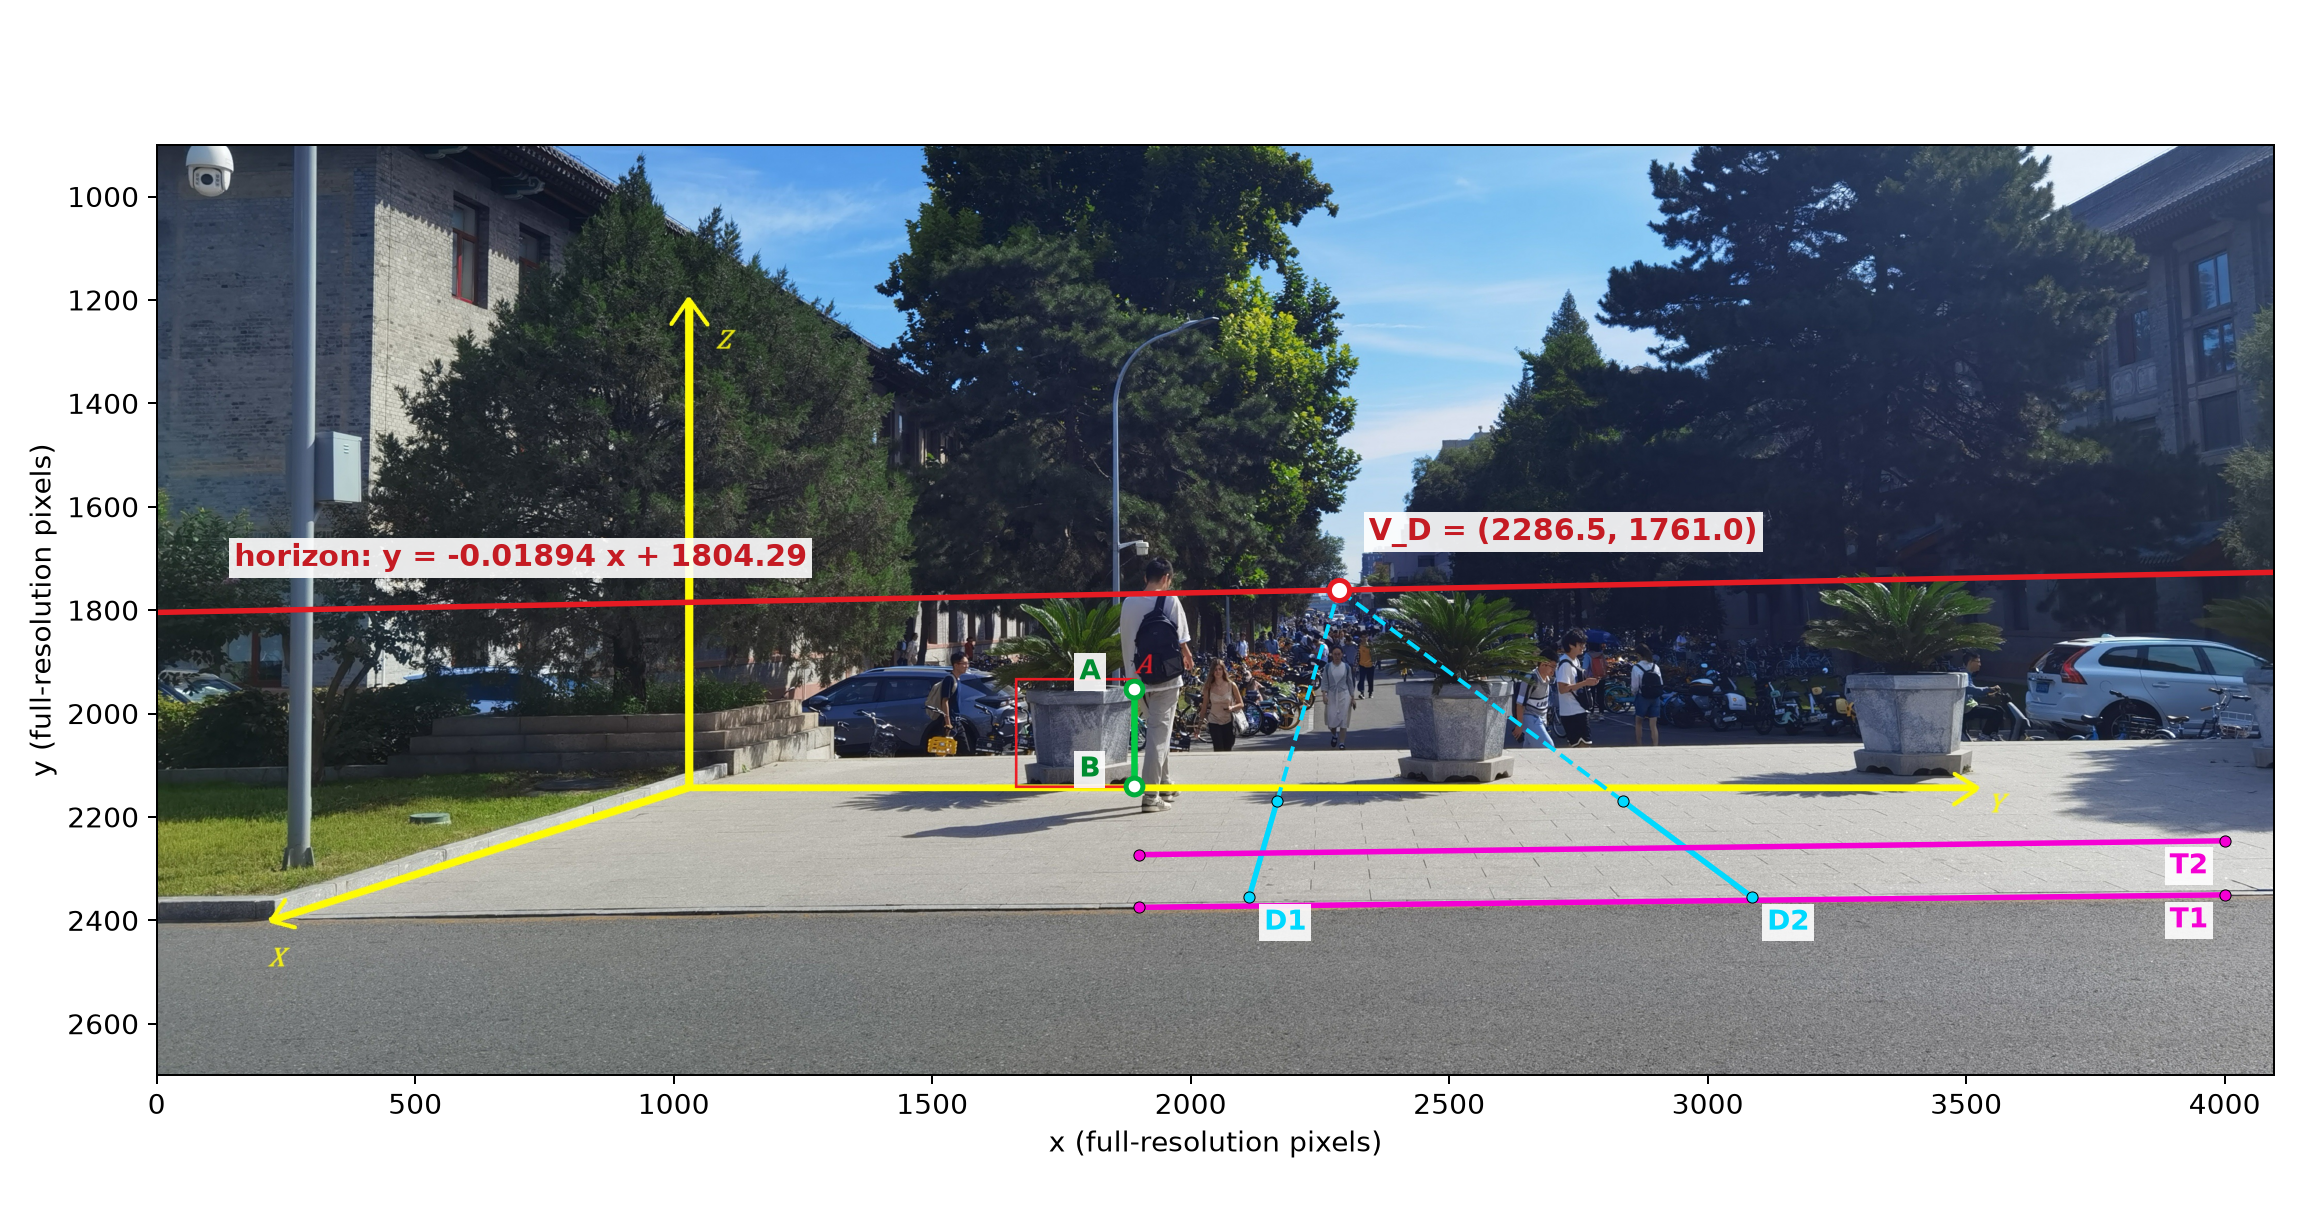
\includegraphics[width=\textwidth]{figs/q2_overview.png}
\caption{平行线与消失线的构造（仅展示原图的局部高度范围，坐标仍为原图坐标）。
青色纵深线的虚线延长部分交于 $V_D$，品红色横向线的交点 $V_T$ 在画幅外；
红色消失线通过两个消失点，绿色为花坛参考高度 $AB$。}
\label{fig:ov}
\end{figure}

\clearpage
\subsection{由参考高度估计相机高度}

\textbf{参考点与局部消失线。} 在全分辨率图像上读取花坛顶沿点 $A=(1891,1953)$，
并按题设近水平近似取其下方的地面点 $B=(1891,2141)$，点位有数像素的测量不确定性。
以 $x_A=1891$ 代入消失线方程：
\begin{equation}
y_h(x_A)=1804.2908-0.0189411\times1891\approx1768.47\ \text{px}.
\end{equation}
故消失线到 $A$ 的距离 $h_1=1953-1768.47=184.53$ px，
$A$ 到 $B$ 的距离 $h_2=2141-1953=188$ px；真实参考高度为 $h=0.76$ m。

\textbf{高度推导。} 设相机离地高 $H$、像素焦距 $f$。在题设水平近似下，
$A,B$ 深度同为 $Z$，高度分别为 $h,0$，针孔模型给出
\begin{equation}
v_B=\frac{fH}{Z},\qquad v_A=\frac{f(H-h)}{Z},\qquad
\frac{v_A}{v_B}=\frac{H-h}{H}.
\end{equation}
消去 $f,Z$，并用 $v_A=h_1$、$v_B=h_1+h_2$，得
\begin{equation}
\boxed{\,H=h\cdot\frac{v_B}{v_B-v_A}=h\cdot\frac{h_1+h_2}{h_2}\,}
\end{equation}
代入 $h_1+h_2=372.53$ px、$h_2=188$ px：
\begin{equation}
H\approx0.76\times\frac{372.53}{188}=1.506\ \text{m}
\quad\Longrightarrow\quad\boxed{H\approx1.5\ \text{m}.}
\end{equation}

\textbf{合理性与误差。} 换用另两条纵深接缝，消失点纵坐标为约 $1751$--$1758$ px，
与 $1760.98$ px 接近。若局部消失线偏差 $20$ px，高度变化约 $0.76\times20/188=0.081$ m。
消失线约 $1.09^\circ$ 的倾斜对应 $AB$ 范围内约 $3.6$ px 横向偏移，
与点位精度同量级。考虑接缝拟合、远处消失点及相机近水平近似的误差，结论取约 $1.5$ m。

\begin{figure}[H]
\centering
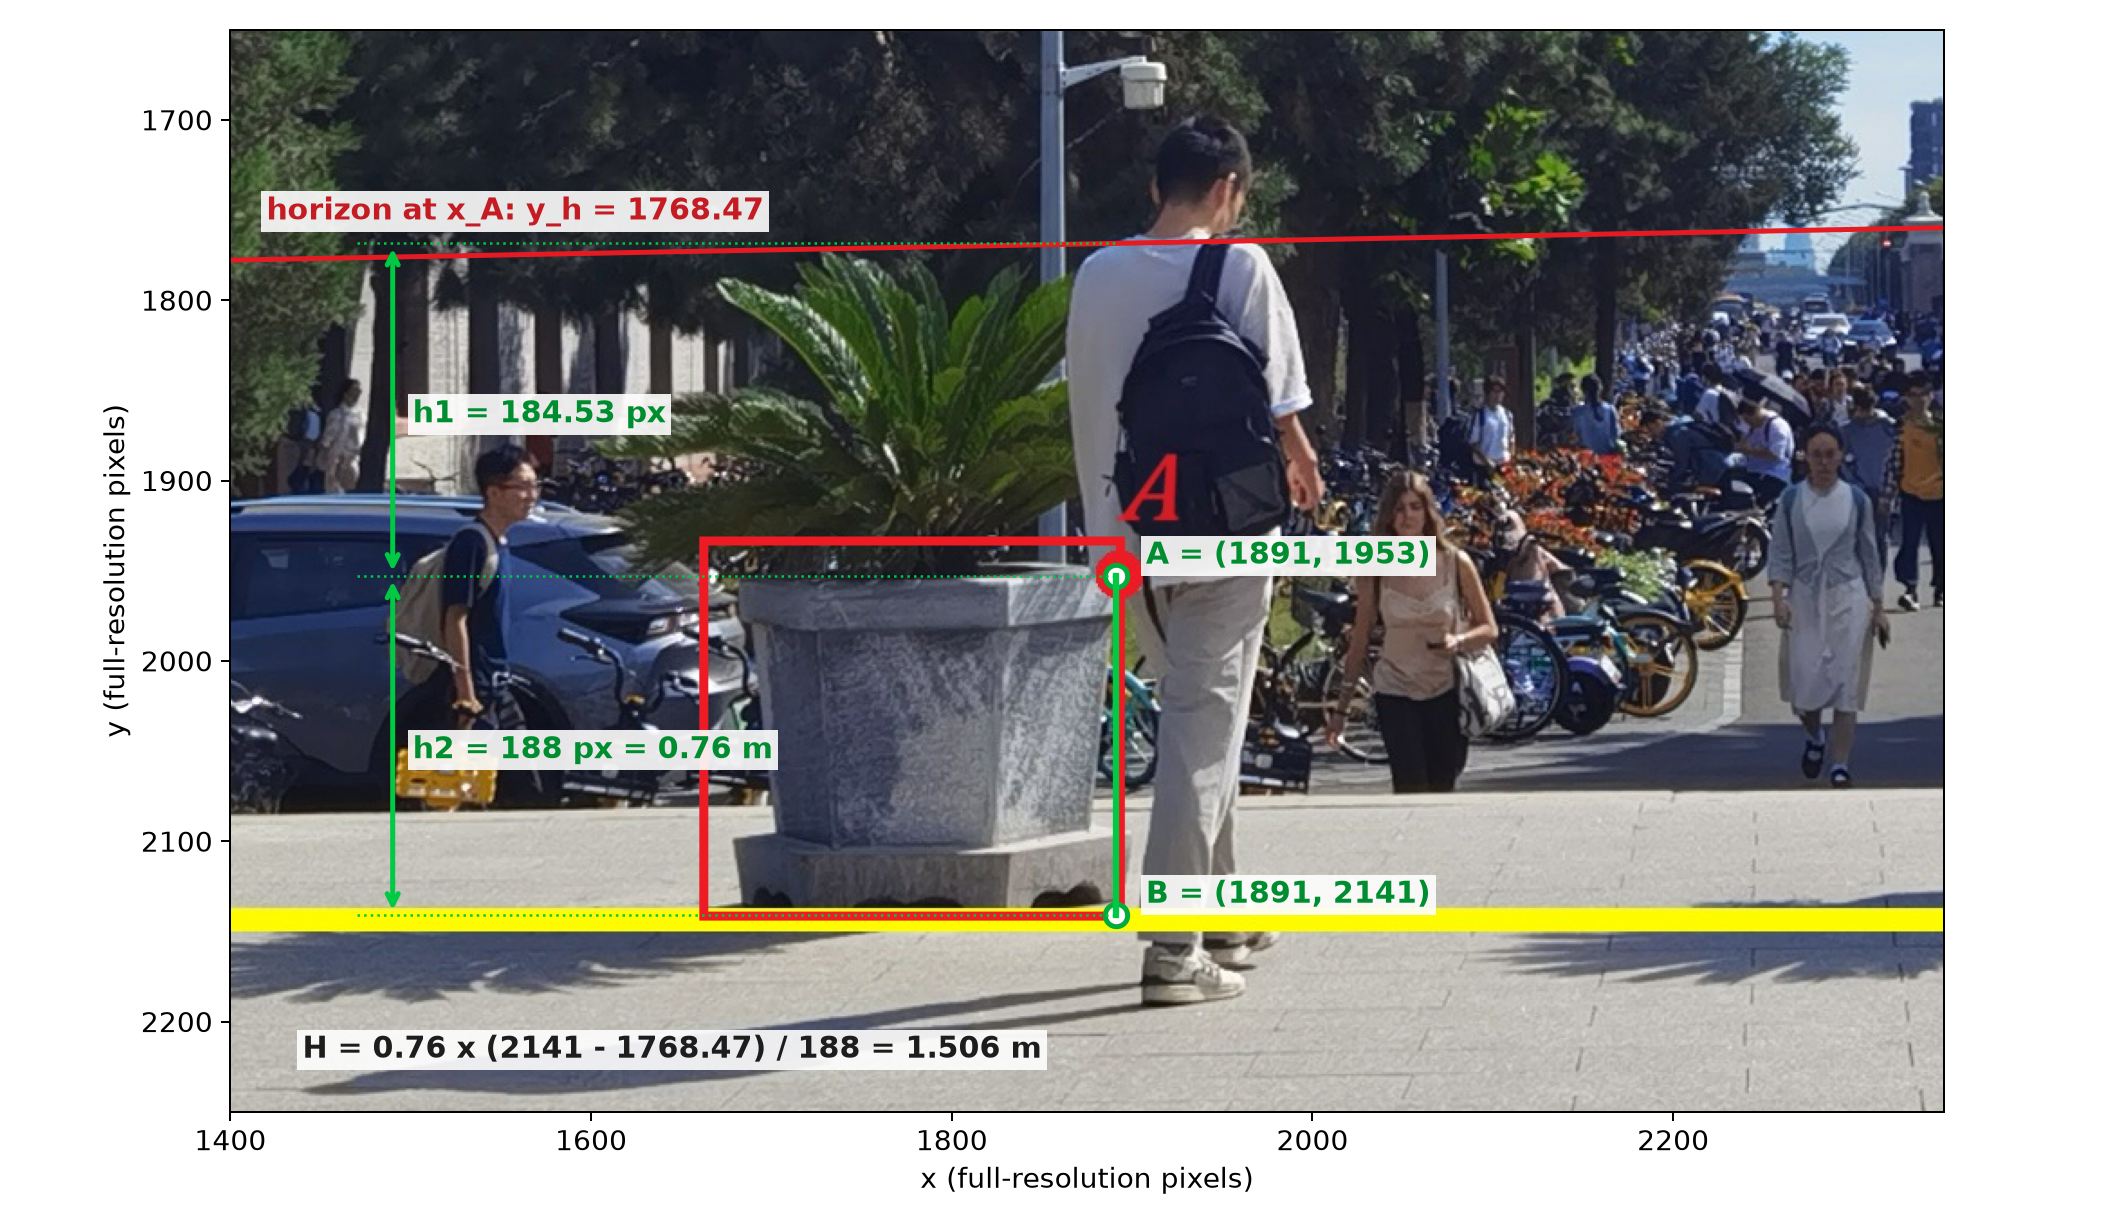
\includegraphics[width=0.78\textwidth]{figs/q2_zoom.png}
\caption{$A$、$B$ 与消失线（局部放大）。$A=(1891,1953)$ 在花坛顶沿上，$B=(1891,2141)$ 是 $A$ 正下方的地面点，
二者对应的真实距离为花坛高度 $0.76$ m；花坛所在列的消失线为 $y_h\approx1768.47$ px，
$h_1\approx184.53$ px，$h_2=188$ px，$H=0.76\,(h_1+h_2)/h_2\approx1.5$ m。}
\label{fig:zoom}
\end{figure}

\clearpage
\section{图像滤波与降采样}

\subsection{实现说明}

所有函数均由本人用 NumPy 实现：

\begin{itemize}
  \item \texttt{cross\_correlation\_2d}$(f,h)$：不翻转核，按
        $g(i,j)=\sum_{k,l} f(i+k,\,j+l)\,h(k,l)$ 逐位移加权求和（用 \texttt{np.pad} 做边界填充）；
  \item \texttt{convolve\_2d}$(f,h)$：把核的两个轴都翻转后调用相关函数，即
        $g(i,j)=\sum_{k,l} f(i-k,\,j-l)\,h(k,l)$；
  \item \texttt{gaussian\_blur\_kernel\_2d}$(k,\sigma)$：$h(x,y)=\frac{1}{2\pi\sigma^{2}}
        e^{-(x^{2}+y^{2})/(2\sigma^{2})}$，$(x,y)$ 取 $[-\frac{k-1}{2},\frac{k-1}{2}]$ 的整数网格，并归一化使和为 $1$；
  \item \texttt{low\_pass}：用上面的核与 \texttt{convolve\_2d} 卷积（另提供可分离版本 \texttt{low\_pass\_separable} 作一致性检查，
        两者最大绝对差 $2.0\times10^{-13}$，仅为浮点舍入误差）；
  \item \texttt{image\_subsampling}$(f,s)$：按因子 $s$ 丢弃行与列，即 $f[::s,::s]$；当尺寸可被 $s$ 整除时为 $(M/s)\times(N/s)$，否则切片保留末尾采样点，尺寸向上取整；
  \item \texttt{gaussian\_pyramid}：每一级先低通、再以因子 $2$ 降采样，得到原图及约 $1/2,1/4,1/8$ 分辨率的四级。
\end{itemize}

\textbf{依赖与运行方式：} 需要 \texttt{numpy}（数组运算）、\texttt{Pillow}（读写图像）、\texttt{matplotlib}（输出对比图）。
在脚本所在目录下运行
\begin{lstlisting}
python3 gaussian_pyramid.py                      # 默认输入 ./zebra.jpg，输出到 ./out
python3 gaussian_pyramid.py --image zebra.jpg --outdir out --kernel 5 --sigma 1.0
\end{lstlisting}
输入输出均使用相对路径，输出目录为 \texttt{./out/}。

子目录为 \texttt{gaussian\_pyramid/}（高斯）与 \texttt{direct\_pyramid/}（直接）。
两者均保存 $1/2,1/4,1/8$ 各级图像；对比图为 \texttt{./out/comparison.png}。

\subsection{滤波金字塔与直接降采样的对比}

对同一张纹理图像 \texttt{zebra.jpg}（$534\times400$，RGB 三通道，未转灰度）分别构造
(a) 高斯金字塔：每级先做 $5\times5,\ \sigma=1.0$ 的高斯低通再隔行隔列抽样；
(b) 直接金字塔：每级直接隔行隔列抽样，不做任何平滑。

\begin{table}[H]
\centering
\caption{两个金字塔对应级别之间的差异（逐像素绝对差），以及各级的高频能量
（HF $=$ Laplacian 绝对值的均值，数值越大高频成分越多）。}
\small
\setlength{\tabcolsep}{5pt}
\begin{tabular}{lcccccc}
\toprule
级别 & 尺寸 & MAE & 最大绝对差 & $>$16 的比例 & HF（高斯） & HF（直接）\\
\midrule
$1/2$     & $267\times200$ & 6.53  & 83.1  & 9.4\%  & 18.58 & 41.78\\
$1/4$     & $134\times100$ & 12.42 & 126.4 & 23.1\% & 21.60 & 60.96\\
$1/8$     & $67\times50$   & 18.87 & 116.6 & 35.2\% & 21.64 & 85.47\\
\bottomrule
\end{tabular}
\end{table}

\textbf{结论：本次实验中两者明显不同，且差异随层数增大。} 目视对比（图 \ref{fig:cmp}）可以看到：
高斯金字塔的各级图像平滑、结构完整；而直接降采样得到的图像出现了明显的锯齿、摩尔纹，分辨率越低越严重
（$1/8$ 级最明显）。定量地看，直接降采样结果的高频能量在每一级都远高于高斯金字塔（$1/8$ 级为 $85.5$ 对 $21.6$），
且与高斯的逐像素差异（MAE $6.53\to18.87$，$>$16 的像素从 $9.4\%$ 升到 $35.2\%$）随层数单调增大。

\textbf{原因（混叠）。} 
\texttt{zebra.jpg} 的条纹本身含有大量接近像素级的高频成分。隔行隔列抽样不会使高频分量消失，而是\textbf{折叠}到低频，
在图像中表现为原来不存在的粗条纹、摩尔纹和锯齿。
高斯低通滤波衰减超出降采样后奈奎斯特频率的分量，从而减轻混叠，但有限大小的高斯核不保证完全消除混叠。
本次直接降采样中，条纹随分辨率降低产生更明显的混叠，对应级别的差异也增大；
这一趋势是本图像的实验结果，并非对所有输入图像都成立。

\begin{figure}[H]
\centering
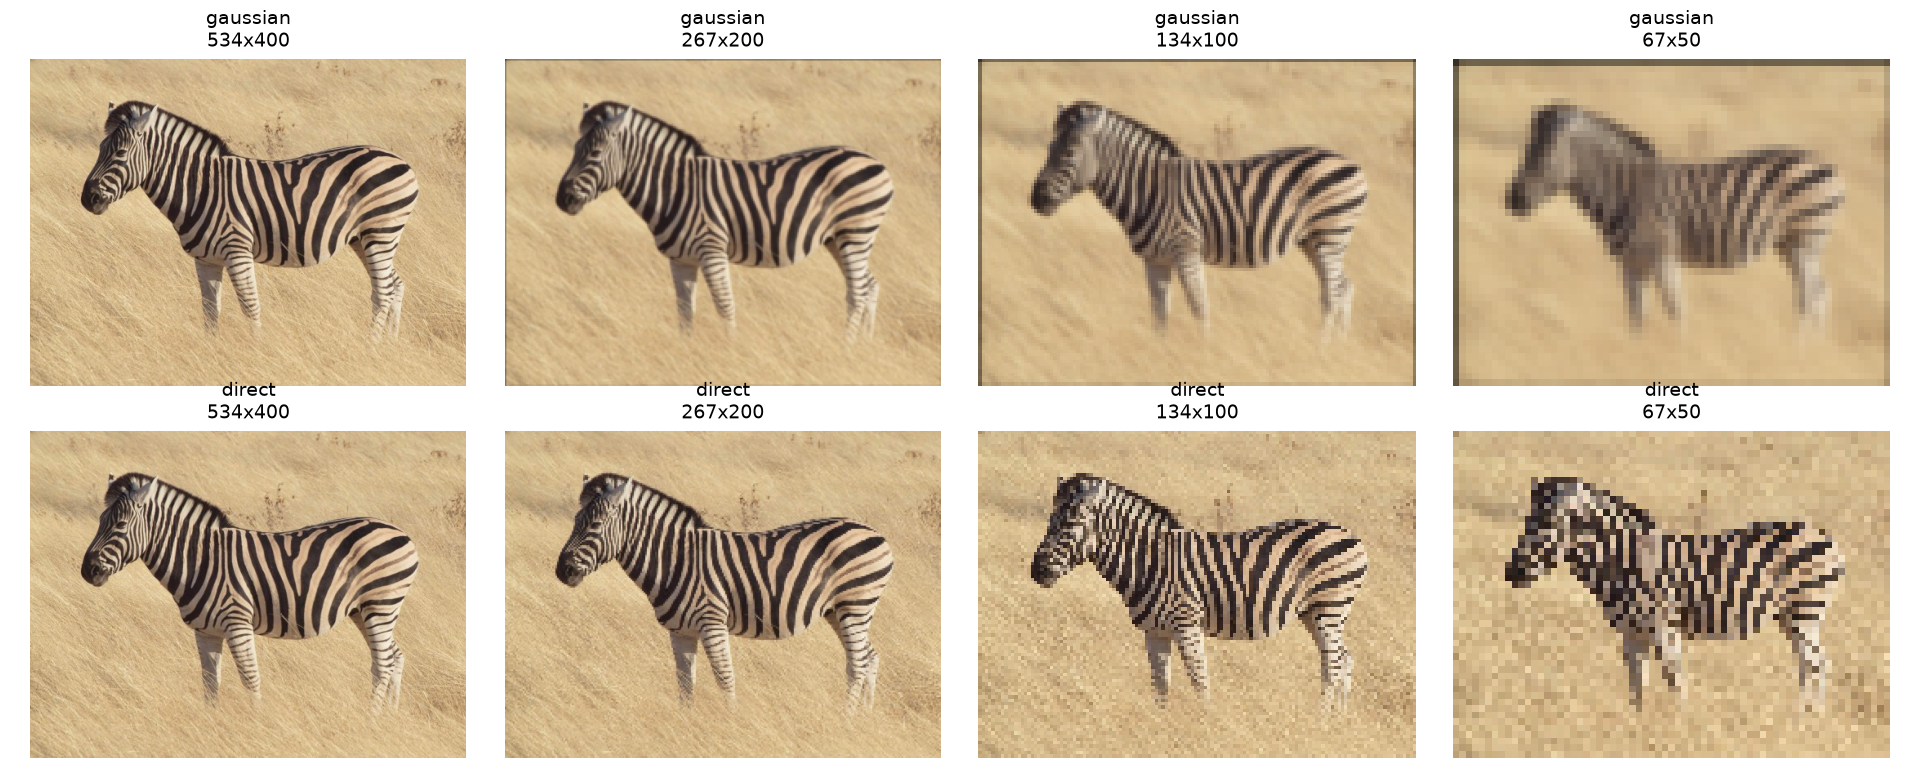
\includegraphics[width=\textwidth]{figs/q3_comparison.png}
\caption{上排为高斯金字塔（先低通再降采样），下排为直接降采样金字塔。
直接降采样各级（尤其 $1/4$、$1/8$）出现明显的锯齿与摩尔纹，即混叠伪影。}
\label{fig:cmp}
\end{figure}

\section{AI 使用声明}

\begin{itemize}
  \item 第 1 题（齐次坐标、卷帘快门）的初稿由本人完成，AI 协助将其手写稿整理为 \LaTeX{} 排版；
        本次修订中 AI 辅助复核并修正了少量表述。
  \item 第 2 题的平行线选择、全分辨率像素测量、消失点与消失线计算、
        相机高度估计、图示及文字修订借助 AI 辅助完成。计算仅使用平行线与题目给定的花坛高度，未使用假定行人身高。
  \item 第 3 题中第 3.1--3.4 节要求的六个函数由本人实现，
        即 \texttt{cross\_correlation\_2d}、\texttt{convolve\_2d} 等六个滤波与金字塔函数；
        \texttt{main()} 中的API接口和调用代码由 AI 协助完成。
  \item 本报告的 \LaTeX{} 排版及本次修订的数值一致性、代码运行和页面显示检查由 AI 协助完成。
\end{itemize}

\end{document}
